\renewcommand{\appendixtocname}{Anexo III}
\appendix
\clearpage
 \addappheadtotoc % Creo que esta linea puede ser eliminada, sino, descomentar y cargar paquete \usepackage[nottoc,notlot,notlof]{tocbibind}
%\appendixpage
\chapter*{ Anexo III} 
En este anexo se presentan los gr\'aficos correspondientes a los modelos Bimodales no estratificados del apartado 5.4.2. En las figuras se observa la distribuci\'on de fuerza promedio de los granos finos y de los granos gruesos.\\

\begin{figure}[htb]
\centering
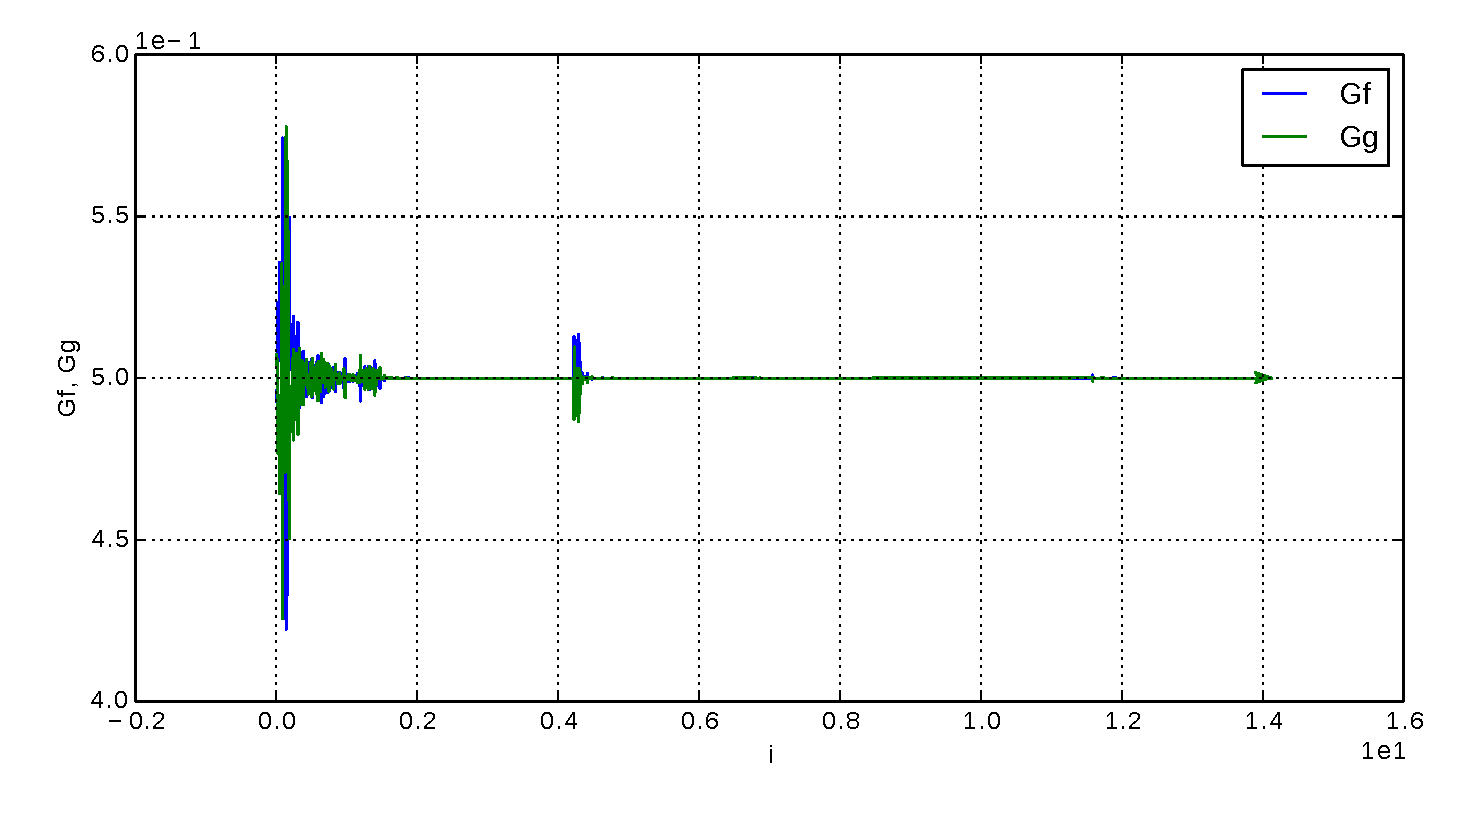
\includegraphics[width=\textwidth]{Anexo2/PSD_10}
\caption{Distribuci\'on de fuerzas promedio de granos finos y gruesos para R=1 y Sd=0.0}
\label{fig:PSD10}
\end{figure}

\begin{figure}[htb]
\centering
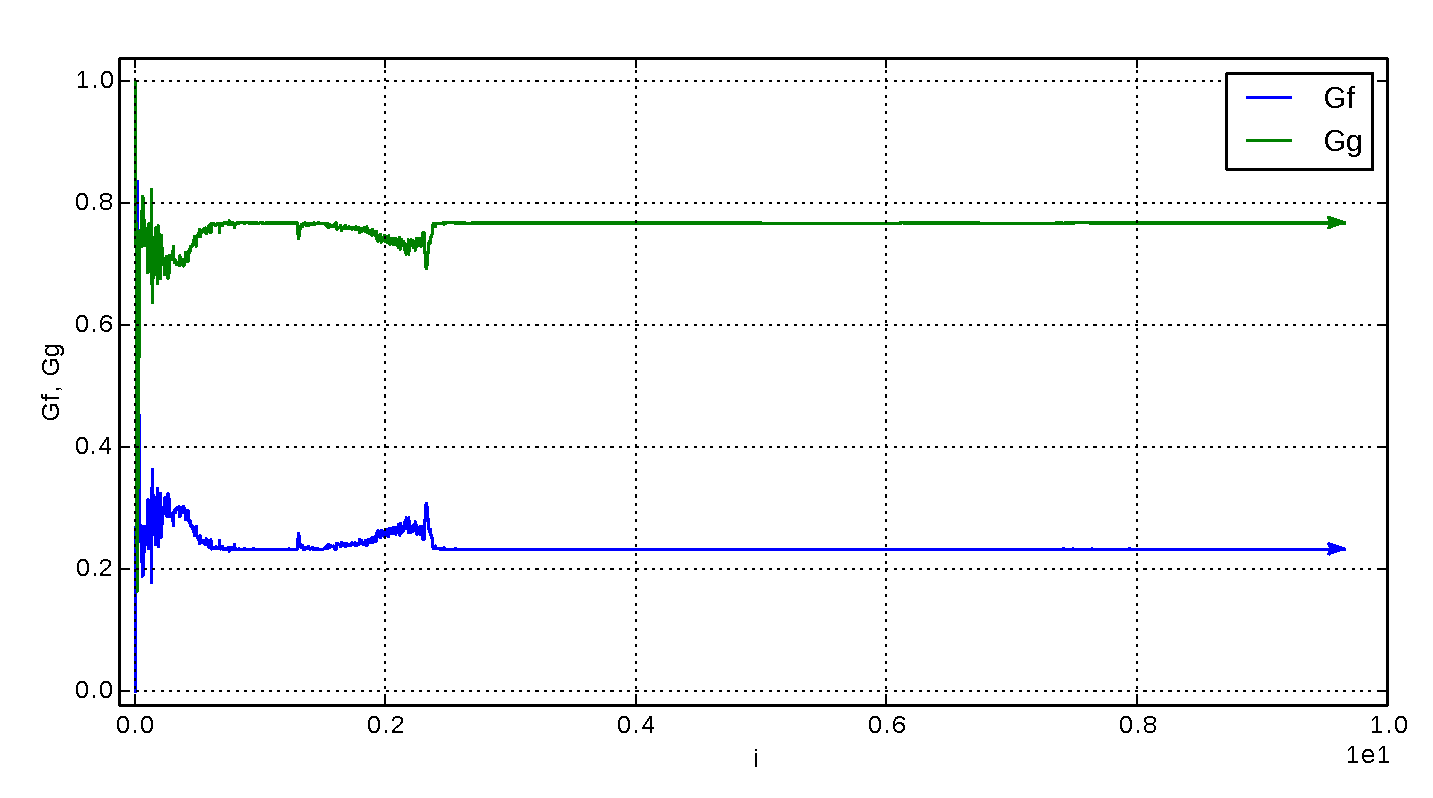
\includegraphics[width=\textwidth]{Anexo2/PSD_15}
\caption{Distribuci\'on de fuerzas promedio de granos finos y gruesos para R=1.5 y Sd=0.05}
\label{fig:PSD15}
\end{figure}

\begin{figure}[htb]
\centering
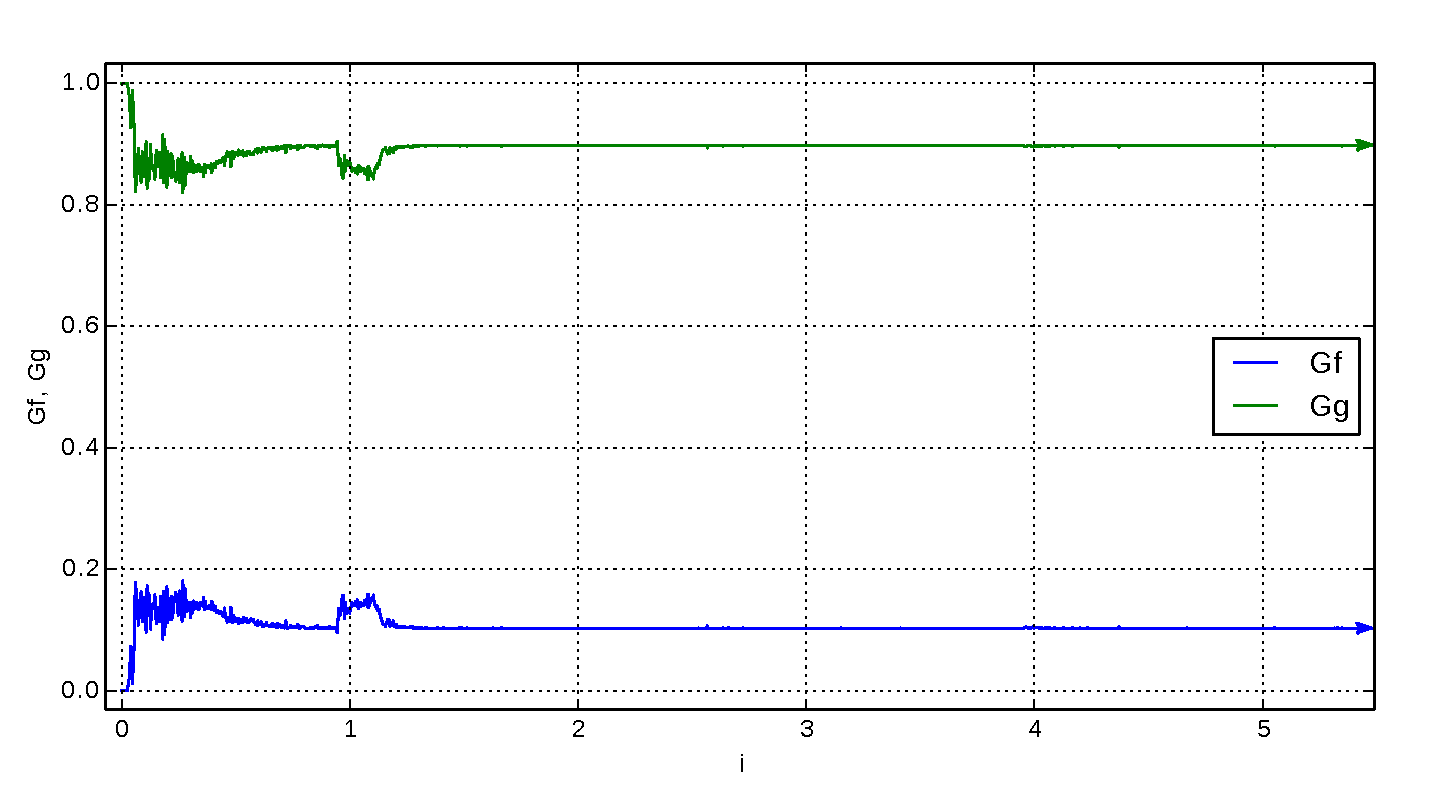
\includegraphics[width=\textwidth]{Anexo2//PSD_20}
\caption{Distribuci\'on de fuerzas promedio de granos finos y gruesos para R=2 y Sd=0.17}
\label{fig:PSD20}
\end{figure}

\begin{figure}[htb]
\centering
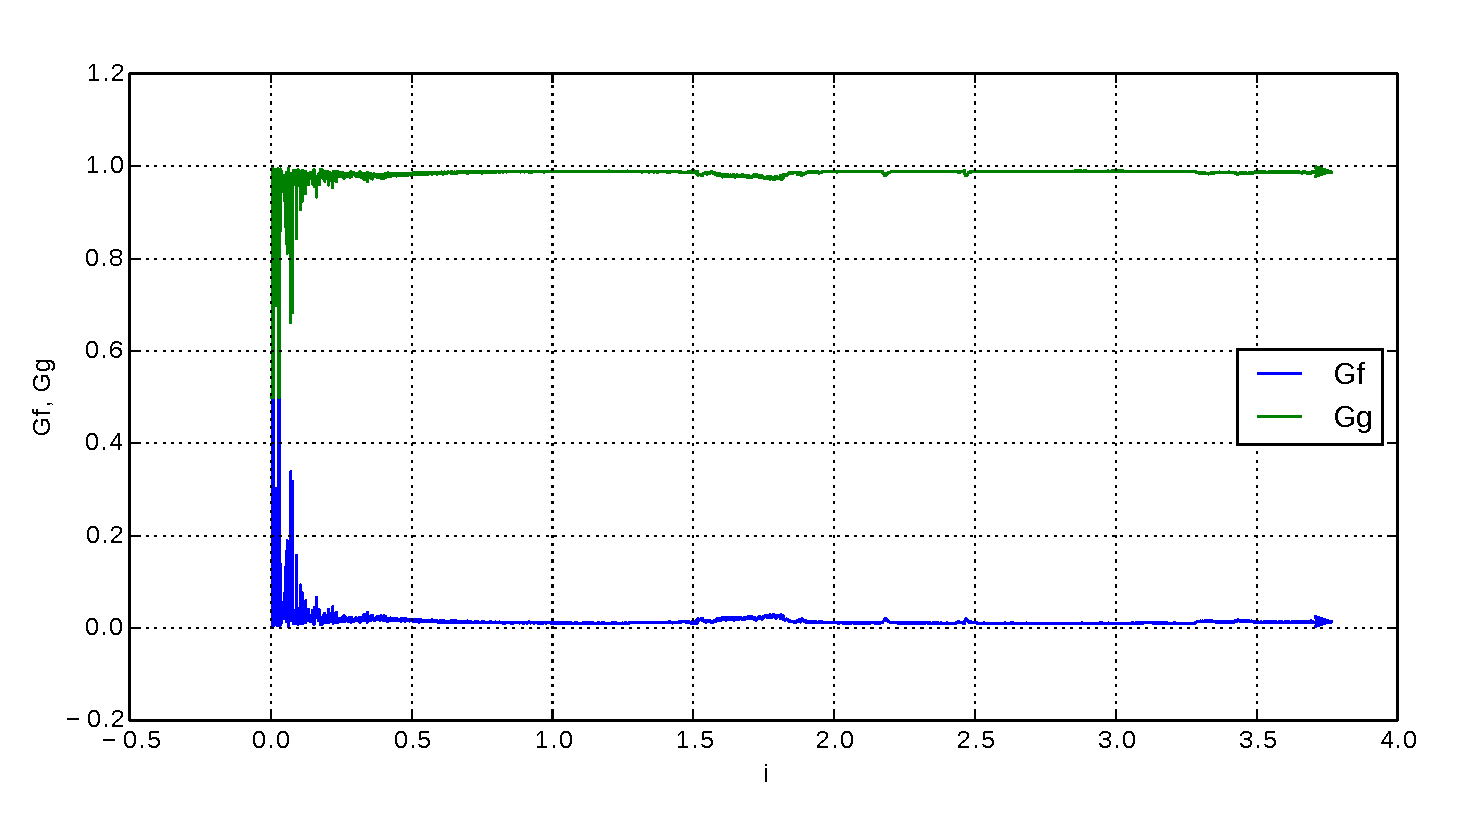
\includegraphics[width=\textwidth]{Anexo2//PSD_46}
\caption{Distribuci\'on de fuerzas promedio de granos finos y gruesos para R=4.6 y Sd=0.51}
\label{fig:PSD46}
\end{figure}


\begin{figure}[htb]
\centering
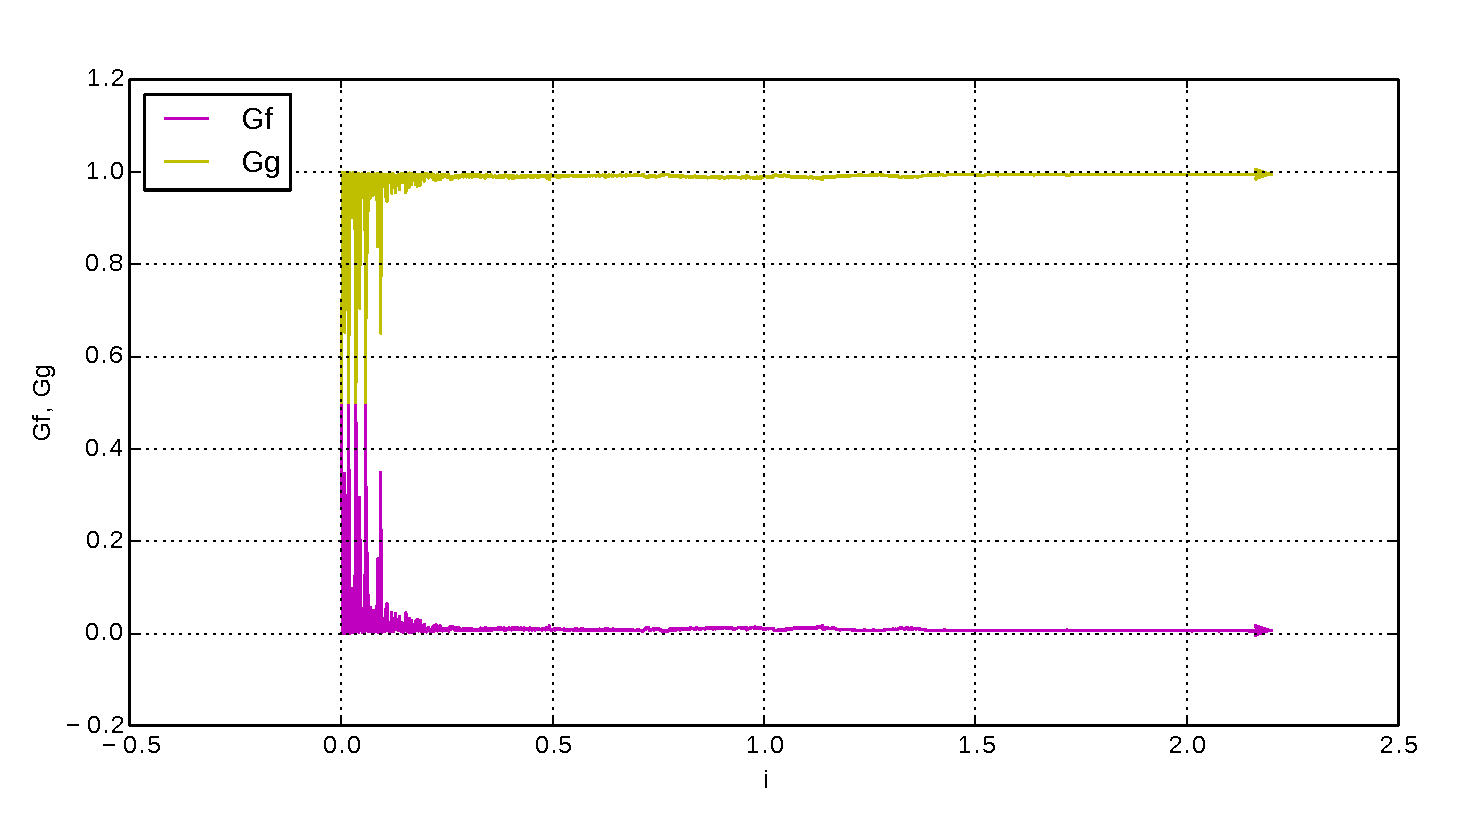
\includegraphics[width=\textwidth]{Anexo2//PSD_50}
\caption{Distribuci\'on de fuerzas promedio de granos finos y gruesos para R=5.4 y Sd=0.68}
\label{fig:PSD50}
\end{figure}









